\documentclass[10pt,oneside,english,a4paper]{article}
\usepackage[english]{babel}
\usepackage[IL2]{fontenc}
\usepackage[utf8]{inputenc}
\usepackage{graphicx}
\usepackage{url} 
\usepackage{hyperref} 
\usepackage{cite}
\usepackage{listings}
\usepackage[margin=3cm]{geometry}

\pagestyle{headings}

\title{How online maps search works: technologies, algorithms and inner structure.
\thanks{Semester project in the subject Methods of engineering work, academic year 2023/24, leadership: PaedDr. Pavol Batalik}}

\author{Anton Dmitriev\\[2pt]
	{\small Slovak University of Technology in Bratislava}\\
	{\small Faculty of Informatics and Information Technologies}\\
	{\small \texttt{xdmitriev@stuba.sk}}
	}

\date{\small \today} 



\begin{document}

\maketitle

\begin{abstract}
	Modern online maps have become an integral part of our daily life, providing us with quick access to geographical information and real-time location. However, behind this wonderful opportunity lies a technically complicated system that has been developing and improving for many years. This article provides an overview of the historical and technological development of online mapping and aims to provide an understanding of how modern online maps function and how they provide users with the data they need. Readers will learn how the evolution of technologies in map data has led to the ability to quickly and accurately find places and addresses on a map. Because, in an era where mobile devices and apps are becoming an essential part of our lives, it is important to understand how these maps collect and store information about the world around us, and how they help us navigate and find the places we need.
\end{abstract}



\section{Introduction}
Since the beginning of exploration of our still undiscovered planet Earth, people have worked hard to record the geographical details of the terrain and the routes of their travels. They did this in order to store information that could be used to further improve navigation (more about the history of cartography in Part 2). The map became a convenient tool for such tasks. However, creating even a single map was a slow and labor-intensive process for the human capabilities of that time. Digital maps, thanks to the ever-increasing availability of computing power, have opened up entirely new possibilities in the field of cartography. Now, after going through this arduous journey of improvements and transformations, a click of the mouse is enough for a computer to plot a user's route from point A to a given point B. "Digital mapping - from the global positioning system (GPS) in your car to the Web site that displays local bus routes - is on the rise"\cite{Mitchell2005}.
\\The Internet, which has become a source for the development of new technologies, provides the average user with just a convenient online map interface. However, not everyone realizes that behind this attractive skin there is a complex mechanism consisting of many interacting high-tech and modern solutions (More about this mechanism in Part~\ref{internal}).


\section{History of online maps development} \label{history}

\subsection{A Brief Background in Cartography} \label{history:brief}
In order to understand modern online maps, it is crucial to delve into the historical roots of cartography. Cartography is a captivating blend of science and art, endeavoring to depict the world as accurately as possible while grappling with the challenge of what to include or leave out. This challenge pertains not only to geographical features but also extends to the selection of a map projection, a pivotal aspect in transforming the spherical Earth into a flat map.
\\Early cartography involved the creation of maps that primarily served navigational purposes. For instance, Polynesian and Micronesian voyagers crafted intricate stick charts to map connections between islands and interpret swell patterns. Portuguese explorers, on the other hand, produced detailed coastal maps that often left the interiors largely blank since their focus was on exploration and seafaring.
\\In 1569, Flemish cartographer Gerardus Mercator introduced a revolutionary map projection\cite{Forrest2021}, which was designed to assist sailors in plotting a straight-line course between any two points. The Mercator projection, or variations thereof, remains the dominant choice in online mapping today due to its ability to depict the entire globe on a nearly square image. However, it comes with a trade-off, introducing size distortions, making it appear as if Greenland is comparable in size to the entire African continent, when in reality, Africa is roughly 14 times larger than Greenland.

\subsection{The First Maps on the Web} \label{history:firstweb}
The emergence of online mapping can be traced back to the early days of the internet. While pinpointing the very first online map is challenging, the transition from static map images to interactive web maps marked a significant milestone. Interactive web maps empowered users, allowing them to control their exploration—zooming in and out, toggling map layers, and more.
\\One of the earliest web maps, the PARC Map Viewer, made its debut in 1993, thanks to Xerox. This pioneering map viewer allowed users to view maps, interact with map features, and toggle map layers. Fundamentally, it operated on a straightforward principle: a user requested a map, the viewer fetched data from a geographic database, rendered a map image, and transmitted it back to the user's browser. This fundamental request-render-return loop remains the core of most web maps today.
\\The PARC Map Viewer was also instrumental in the inception of "mashups." It allowed overlaying data on maps, exemplified by the display of earthquake data facilitated by the World-Wide Earthquake Locator developed by the University of Edinburgh in 1994. This mashup concept gained swift adoption among developers, heralding a new era in web mapping (More about "Mashups" in Part~\ref{history:mashups}).

\subsection{The Rise of Consumer-Facing Web Mapping Services} \label{history:userfriendly}
In 1996, Mapquest and Multimap, both launched in the same year, marked the advent of user-focused web mapping services. These platforms offered users the ability to input their addresses and witness their locations represented on maps, which was a revolutionary concept at the time. Mapquest, in particular, introduced features like zooming and panning, enhancing the interactivity of web maps.
\\User-friendly web mapping services revolutionized navigation by rendering traditional printed road maps increasingly obsolete. The ease of locating oneself and obtaining driving directions online fundamentally reshaped how people navigated the world around them.
\\However, these early web maps had a limitation: every time the map was panned or zoomed, the entire map view had to reload, resulting in a somewhat slow user experience.

\subsection{Google Maps: A Game-Changer} \label{history:gamechanger}
Google entered the web mapping arena and turned the tables in 2005 with the launch of Google Maps. Google Maps incorporated groundbreaking features like satellite imagery and an interactive interface, which garnered rapid popularity. 
\\Key to the success of Google Maps was its use of map tiles, small square images that made up the larger map, and the utilization of the Mercator projection~\ref{history:brief}. These tiles allowed for faster loading times and efficient use of resources. Moreover, Google's innovative map tiles were capable of rendering different zoom levels, further enhancing the user experience. %(more about how tiles works in 3 или 4 или 5 или отдельно я не ебу)
\\Google Maps didn't stop at providing directions but went a step further by introducing a blue dot to indicate a user's precise location. This feature opened the door to a new industry centered around location, with services like Foursquare and Yelp leveraging location data for various purposes, from reviews to recommendations.

\subsection{Terravision: A Pioneering 3D World Mapping Software} \label{history:patentrights}
It would seem that we all know the most popular online mapping service such as Google Maps (originally Google Earth). But there were some dark places in its history of creation. Terravision\cite{Leclerc1994} was a one of the firs 3D world mapping software program developed by a group of German university students from ART+COM, including Jachim Sauter and Juri Muller. Launched in 1993, Terravision aimed to provide a networked, virtual, and graphical representation of Earth using 3D graphics. Juri Muller, as the chief programmer, was responsible for inventing the algorithms that powered the software. Joachim Sauter, on the other hand, focused on the program's design and artistic elements. The result was a unique fusion of art and technology.
\\Terravision quickly gained worldwide attention in the early '90s, as it was a novel concept not seen in the technology and internet landscape of that time. During the exhibition tours, the creators of Terravision made a visit to Silicon Valley, where Juri Muller accidentally told the details of Terravision's algorithms to Brian McClendon, an American software engineer and skilled programmer.Brian used this information to develop in collaboration with Google a program that would later become a household name in the field of online mapping, "Google Earth".
\\In 2014, ART+COM, the company responsible for Terravision, filed a lawsuit against Google, alleging that Google's product, Google Earth, infringed upon the patent rights of Terravision, which had been invented in 1993. Two years later, the legal dispute reached its resolution: The United States District Court for the District of Delaware ruled in favor of Google.
\\The legal clash between Terravision and Google attracted significant attention and ultimately became the subject of a Netflix series titled "The Billion Dollar Code."

\subsection{Mashups and the Emergence of OpenStreetMap} \label{history:mashups}
While Google Maps was gaining momentum, developers were beginning to explore the idea of integrating their own data into web maps. This was exemplified by Paul Rademacher, who ingeniously used unsanctioned APIs from Google Maps to create HousingMaps.com, a platform that combined Craigslist rental listings with Google Maps. This represented the birth of mashup mapping, which allowed users to overlay their data onto established web map services.
\\Instead of shutting down these mashups, Google embraced the trend by introducing the Google Maps API, which made it possible for developers to utilize Google Maps as a service for their applications. This step effectively commercialized the mapping product.
\\The idea of overlaying data on web maps and the popularity of Google Maps inspired a new generation of mapping services and projects. Notably, OpenStreetMap (OSM) , launched in 2004, gained traction by inviting users to add or edit map features, such as roads, waterways, and points of interest. OSM, often described as the "Wikipedia for maps," fostered a global community of contributors, leading to a significant increase in data quality and coverage.

\subsection{Vector Tiles and the Democratization of Mapping Data} \label{history:vector}
The transformation of web maps continued with the introduction of vector tiles, a significant leap forward in technology. Unlike traditional map tiles that consist of static images, vector tiles contain raw geospatial data that can be rendered in real-time by the browser. This shift made maps more dynamic, allowing for smoother and more interactive map experiences.
\\Vector tiles were especially well-suited for the mobile environment and were made possible through technologies like WebGL, which enhanced graphics rendering in browsers. This innovation allowed developers to create map-based applications with greater efficiency and flexibility.
\\Web mapping saw a pivotal moment when Uber sought to visualize its extensive ride data. Faced with vast amounts of ride records, Uber embarked on the development of tools that could efficiently handle and visually represent massive datasets. One of the outcomes was Deck.gl, a framework for rendering large-scale data visualizations on maps. This open-source project opened doors for data visualization in various fields, from urban planning to spatial analytics.

\section{Internal structure} \label{internal}

\subsection{Shortest Path from Point A to Point B} \label{internal:dijikstra}
Google Maps utilizes graph data structures to compute the shortest route from a source point (point A) to a destination (point B). A graph data structure is composed of numerous nodes interconnected by multiple edges. Edsger W. Dijkstra introduced the Dijkstra's algorithm, an efficient method for determining the shortest distance and path to a specified destination. In this graph, nodes are linked by weighted edges, which signify the distance required to travel to each node. 
\\Here's how this algorithm works\cite{Mehta2019}:

\begin{enumerate}
	\item Choose an initial node in the weighted graph which serves as a source node.
	\item The distance of the other nodes is intialised as infinity with respect to the source node. 
	\item An empty set N containns the nodes to which the shortest path has been found. 
	\item The distance of the source node with respect to itself is zero. It is added to N and thus termed as ‘active node’. 
	\item Consider the neighbouring nodes of the active node which are connected to it by a weighted edge. Sum up the distance with the weight of the edge. 
	\item If the neighbouring nodes already have some distnace assigned, then update the distance if the newly obtained distance in step 5 is less than the current value. 
	\item Now, choose the node which has the minimum distance assigned to it and insert it into N. The newly inserted node is now the ’active node’. 
	\item Repeat steps 5 to 7 until the destination node is included in the set N or if there are no more labelled nodes in N.
	
\end{enumerate}

\begin{lstlisting}[language=C++, caption=Pseudo code representation, frame =single, basicstyle=\ttfamily\small]
function  dijkstraAlgorithm(graph, source):
	for each node n in graph:
		distance[n] := infinity
		previous[n] := undefined
	distance[source] := 0
	q := the set of all nodes in graph
	while q is not empty:
		z := node in q with smallest distance[ ]
		remove z from q
		for each unvisited neighbor n of z:
			dist := distance[u] + dist_between(z, n)
			if dist < distance[n]
				distance[n] := dist
				previous[n] := z
return distance[ ] previous[ ]

\end{lstlisting}
In the context of Google Maps, this graph represents the road network, with each road segment serving as a node and intersections as the connecting points. While the Dijkstra's algorithm may lose its efficiency when dealing with the big data of Google Maps, it still forms the foundational concept of the algorithm that modern online maps rely upon to determine the shortest path between two points.

\subsection{What is Geocoding?} \label{internal:geocoding}
Geocoding is a fundamental component of spatial analysis that has found applications across various research disciplines and domains. It involves the process of converting descriptive locational data, such as postal addresses or named places, into absolute geographic references. Over the years, geocoding has undergone significant evolution, transforming from a costly and limited practice to a more accessible and accurate method, often available for free through online services \cite{Goldberg2007}. 
\\Early geocoding systems, like those used by the U.S. Census in the 1960s, primarily assigned numerical codes to postal addresses and named buildings, resulting in low-resolution geographic output. Then the idea of geocoding was extended in the early 20th century with the development of automobile navigation systems. The main challenge was to develop a way to convert textual descriptions of addresses (e.g., "1010 E Main St, Waynesboro, VA 22980, USA ") into numerical coordinates (38.064050, -78.873830) that could be used for navigation. This first became widely available through the Global Positioning System (GPS) in the late 20th century.
\\Geocoding is based on mapping text addresses to geographic coordinates. The process involves the following steps \cite{Behr2010}:

\begin{enumerate}
\item Receiving the request: The user enters a textual description of the location into the search box or through the map interface.
\item Analyzing the query: The server analyzes the request, trying to understand what type of location is specified (e.g., address, place name, zip code, etc.).
\item Database Search: The server accesses its geographic database, which contains information about millions of locations. It looks for a match between the query entered and the data in the database.
\item Result ranking: The server returns a list of the most likely results ranked by similarity to the request. 
\item Geographic coordinates output: The server returns the geographic coordinates (latitude and longitude) of the selected location.
\item Display on map: The received coordinates are used to display the selected location on the map. The map is centered on that location and information about the location is shown to the user.
\end{enumerate}

\begin{figure}[h]
	\centering
	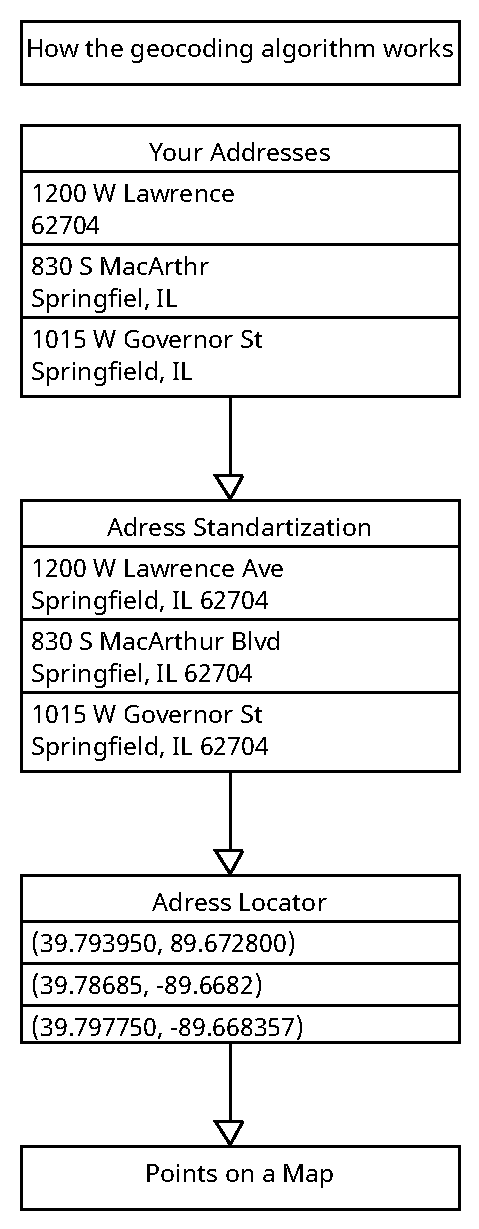
\includegraphics[scale=0.5]{diagram1.pdf}
	\caption{Process of Geocoding}
	\label{fig:geocoding}
\end{figure}

So modern online maps make extensive use of geocoding to provide location information and navigation. Here are a few scenarios of how geocoding is used in modern online maps:

\begin{itemize}
\item Searching and finding places.: Geocoding allows online map users to find places by address or keywords. A user can type in the name of a restaurant, store, or address, and online maps will convert that query into coordinates and display the location on the map.
\item Navigation and route creation: When creating routes between two points, geocoding is used to determine the coordinates of the start and end points and to find the best route between them.
\item Information about nearby objects: Maps use geocoding to provide information about nearby objects such as restaurants, hotels, gas stations, and other establishments. The user can see their location on the map and get more information about them.
\item Geotagging of photos: If a user takes a photo of a location using a mobile device, the phone can use geocoding to automatically add location coordinates to the photo. This allows users to organize and find photos by location.
\end{itemize}

Geocoding plays an important role in the functionality of modern online maps, making it a powerful tool for navigating, finding places, and getting information about geographic locations. Accurate geocoding can greatly enrich the user experience and help find information about the world around them. 

\subsection{Location Detection: You Can't Hide from It} \label{internal:gps}


\bibliography{literatura}
\bibliographystyle{plain}
\end{document}
